\documentclass[xcolor=dvipsnames]{beamer}%[hyperref={pdfpagelabels=false}]{beamer}

\usepackage{polski}
\usepackage[utf8]{inputenc}
\usepackage{caption}

\usepackage{lmodern}
\usepackage{amsfonts}
\usepackage{hyperref}
\usepackage{amsmath}
\usepackage{graphicx}
\usepackage{pdflscape}
\usepackage{subfigure}
\usepackage{appendixnumberbeamer}

\usepackage{makecell}
\usepackage{multicol}
\usepackage{amsmath}

\usepackage{pgf}
\usepackage{eso-pic}
% \usepackage{enumitem}

\renewcommand\theadalign{bc}
\renewcommand\theadfont{\bfseries}
\renewcommand\theadgape{\Gape[4pt]}
\renewcommand\cellgape{\Gape[4pt]}

%%%%%%%%%%%%%%%%Początek ustawień

\definecolor{pwr}{RGB}{154,52,45}
\definecolor{blue_dark}{RGB}{40,66,146}
\definecolor{blue_light}{RGB}{51, 102, 153}

% \setbeamercolor*{sidebar}{fg=blue_dark,bg=blue_light}

\usepackage{beamerthemesplit}
\useoutertheme{infolines}
\useinnertheme{rounded}

\setbeamertemplate{navigation symbols}{}%remove navigation symbols

%%%%%%%%%%%%%%%%%Koniec Ustawień

%%%%%%%%%%%%%%%%% SLAJD TYTUŁOWY

\title[ESTEC, Noordwijk]{\textbf{TRACZ}}
\subtitle{\textbf{T}esting \textbf{R}obotic  \textbf{A}pplications for \textbf{C}atching in \textbf{Z}ero-g} 
\author[Team TRACZ]{Aleksander Gorgolewski \and Aleksander Bojda \and Aleksander Tuzik \and Aleksander Sil \and Adrianna Graja \and Jakub Kielar \and Łukasz Chojnacki \and Maciej Draguła}
\institute[WUST \& UWr]{Wroclaw University of Science and Technology \and University of Wroclaw}


\titlegraphic{%
\vspace{25pt}
\makebox[\textwidth][c]{
    
\includegraphics[height=0.7cm,keepaspectratio]{figure/logo_esa.eps}%
	    \hspace{10pt}
    
\includegraphics[height=0.7cm,keepaspectratio]{figure/logo_SNSB.jpg}%
    	\hspace{10pt}
    
\includegraphics[height=0.7cm,keepaspectratio]{figure/logo_SSC.png}%
        \hspace{10pt}
    
\includegraphics[height=0.7cm,keepaspectratio]{figure/logo_ZARM.jpg}%
        \hspace{10pt}
    
\includegraphics[height=0.7cm,keepaspectratio]{figure/logo_DLR.png}%
        \hspace{10pt}
    
\includegraphics[height=0.7cm,keepaspectratio]{figure/logo_EL.jpg}%
	} 
}

%Mission steatement: TRACZ (Testing Robotic Applications for Catching in Zero-g) is an experiment which aims to investigate a possibility of application universal soft gripper in space conditions.

%%%%%%%%%%%%%%%%%%%%%%%%%%%%%%%%%%%%%%%%%%%%%%%%%%%%%%%%%%%%%%%%%%%%%%%%%%%%%%%%%%%%%%%%%%%%%%%%%%%%%%

\begin{document}

\begin{frame}
\maketitle
\end{frame}


\begin{frame}
\frametitle{Agenda}
\tableofcontents
\end{frame}

%%%%%%%%%%%%%%%%%%%%%%%%%%%%%%%%%%%%%%%%%%%%%%%%%%%%%%%%%%%%%%%%%%%%%%%%%%%%%%%%%%%%%%%%%%%%%%%%%%%%%%

\section{Introduction}

\subsection{Scientific background and technical motivation}        
\begin{frame} %początek slajdu
\frametitle{Motivation}
\framesubtitle{Scientific background and technical motivation} %Opcjonalnie

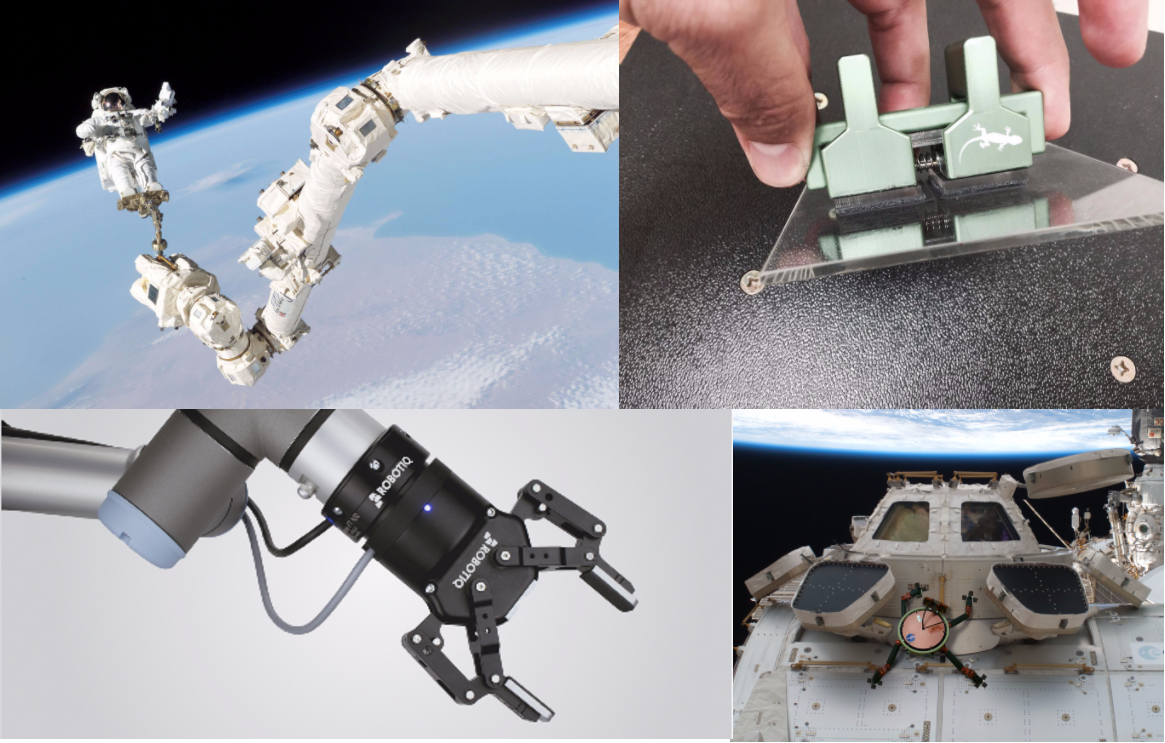
\includegraphics[width=\textwidth]{figure/motivation.png}
\centering   %Universal device which can grab differently shaped and sized                        
%elements made from various materials for space applications    %      %do cięcia - w razie potrzeb, można ten slajd wyrzucić i zawrzeć treść w slajdzie z methods.jpg
% Do wyrzucenia. Nie robi się takich slajdów :) Trzeba to sobie zanotować i mieć w skrypcie prezentacji, żeby to powiedzieć ewentualnie

% Jakis obrazek z projektu GECKO lub czegos innego do chwytania

\end{frame}



\begin{frame} %początek slajdu
\frametitle{Scientific and technical objectives}
\framesubtitle{Scientific background and technical motivation} %Opcjonalnie
\centering
\includegraphics[]{figure/arrow.png}\\
\centering  \textbf{ To test the application of jamming gripper in space conditions} \\
%One of the most challenging parts of the experiment is to 
%Observe how the effector works while gripping an irregular object in                    
%microgravity and vacuum conditions. Observation will be performed     

%by a camera during the whole process of gripping objects. \\ 	
%To measure the grip force of a jamming gripper in space conditions\\
%\vspace{3mm}

%\textbf{Scientific objective no.2} \\
%The second goal is to compare measured maximum grip force                    
%with the experiment carried out on the ground. The comparison will                      
%answer a question: Do space conditions help jamming gripper to                    
%grip objects? 
%To observe the effector behavior in microgravity and vacuum conditions \\
%To calculate grip force of a jamming gripper in space conditions\\
%Determination whether the jamming gripper is feasible/suitable for space applications\\
%Comparison of maximum grip force between Space and ground/Earth conditions\\
%\vspace{3mm}

%\textbf{Scientific objective no.3} \\
%To grab various objects of different sizes, shapes and surfaces
%The second goal is to compare measured maximum grip strength                    
%with the experiment carried out on the ground. The comparison will                      
%answer a question: Do space conditions help jamming gripper to                    
%grip objects? 
%To compare grip strength of a jamming gripper between Space \\
%Determination whether the jamming gripper is feasible/suitable for space applications\\
%Comparison of maximum grip strength between Space and ground/Earth conditions\\
%\vspace{3mm}

%\textbf{Technical objective} \\
%One of the most innovative parts of the experiment is a design and construction of universal jamming gripper, which can operate under                  
%microgravity and vacuum conditions. The gripper should be                
%resistant to harsh conditions of delivery and work in microgravity                    
%and vacuum. Choice of the elastic material for membrane will be                      
%challenging.  
%To construct a universal jamming gripper suitable for microgravity and vacuum environment
\end{frame}

% To test the application of jamming gripper in space conditions

\subsection{Introduction of experiment background} % 


\begin{frame}
\frametitle{Background of the experiment}
  \centering
  \includegraphics[height=7cm]{figure/gripper_google.png}	
%   Tutaj wstawiamy kradzione zdjecie chwytaka i mówimy jak on w ogóle jest skonstruowany (jakieś ladne zeby bylo widac kolnierz, balon i podstawe). Dac podpis skad zdjecie brane.
  
\end{frame}


\begin{frame}
\frametitle{How does it work?}
  \centering
  %Opis dzialania 
  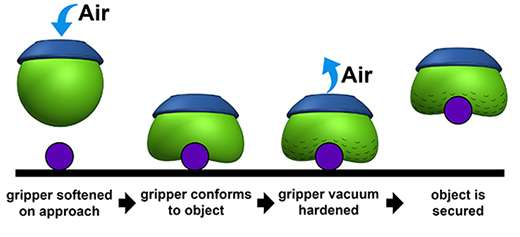
\includegraphics[width=0.75\textwidth]{figure/how_gripper_works.jpg}		
\end{frame}


%\begin{frame} %początek slajdu
%\frametitle{Technical objective}
%\framesubtitle{Scientific background and technical motivation} %Opcjonalnie

%\centering  \textbf{Technical objective} \\
%One of the most innovative parts of the experiment is a design and construction of universal jamming gripper, which can operate under                  
%microgravity and vacuum conditions. The gripper should be                
%resistant to harsh conditions of delivery and work in microgravity                    
%and vacuum. Choice of the elastic material for membrane will be                      
%challenging.  
%\end{frame}


\subsection{Team} % 
\begin{frame} %początek slajdu
\frametitle{Team members}
% \framesubtitle{Introduction of experiment idea and experiment objectives} %Opcjonalnie

\begin{columns}

\column{0.25\textwidth}
\begin{minipage}[c][0.45\textheight][c]{\linewidth}
  \centering
    \begin{table}[H]
    \centering
    \begin{tabular}{c}
    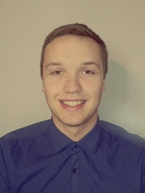
\includegraphics[height=0.2\textheight]{figure/Gorgolewski.jpg}\\
    \textbf{Aleksander}\\\textbf{Gorgolewski}\\
    Project manager
    \end{tabular}
    \end{table}
\end{minipage}
\begin{minipage}[c][0.3\textheight][c]{\linewidth}
  \centering
    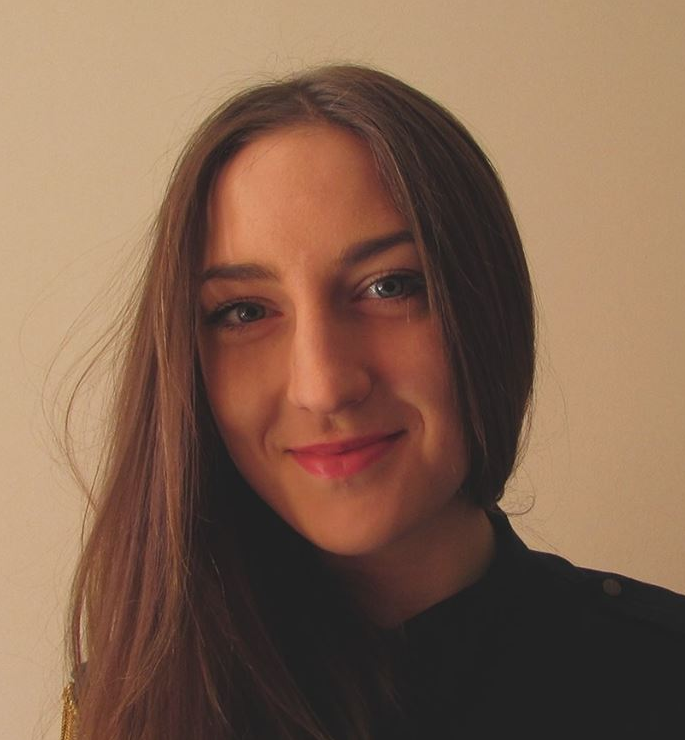
\includegraphics[height=0.2\textheight]{figure/ada.png}\\
    \textbf{Adrianna}\\\textbf{Graja}\\
    Mechanics
  
\end{minipage}

\column{0.25\textwidth}
\begin{minipage}[c][0.45\textheight][c]{\linewidth}
  \centering
    \begin{table}[H]
    \centering
    \begin{tabular}{c}
    
\includegraphics[height=0.2\textheight]{figure/aleksander_sil.jpg}\\
    \textbf{Aleksander}\\\textbf{Sil}\\
    Electronics
    \end{tabular}
    \end{table}
\end{minipage}
\begin{minipage}[c][0.3\textheight][c]{\linewidth}
  \centering
  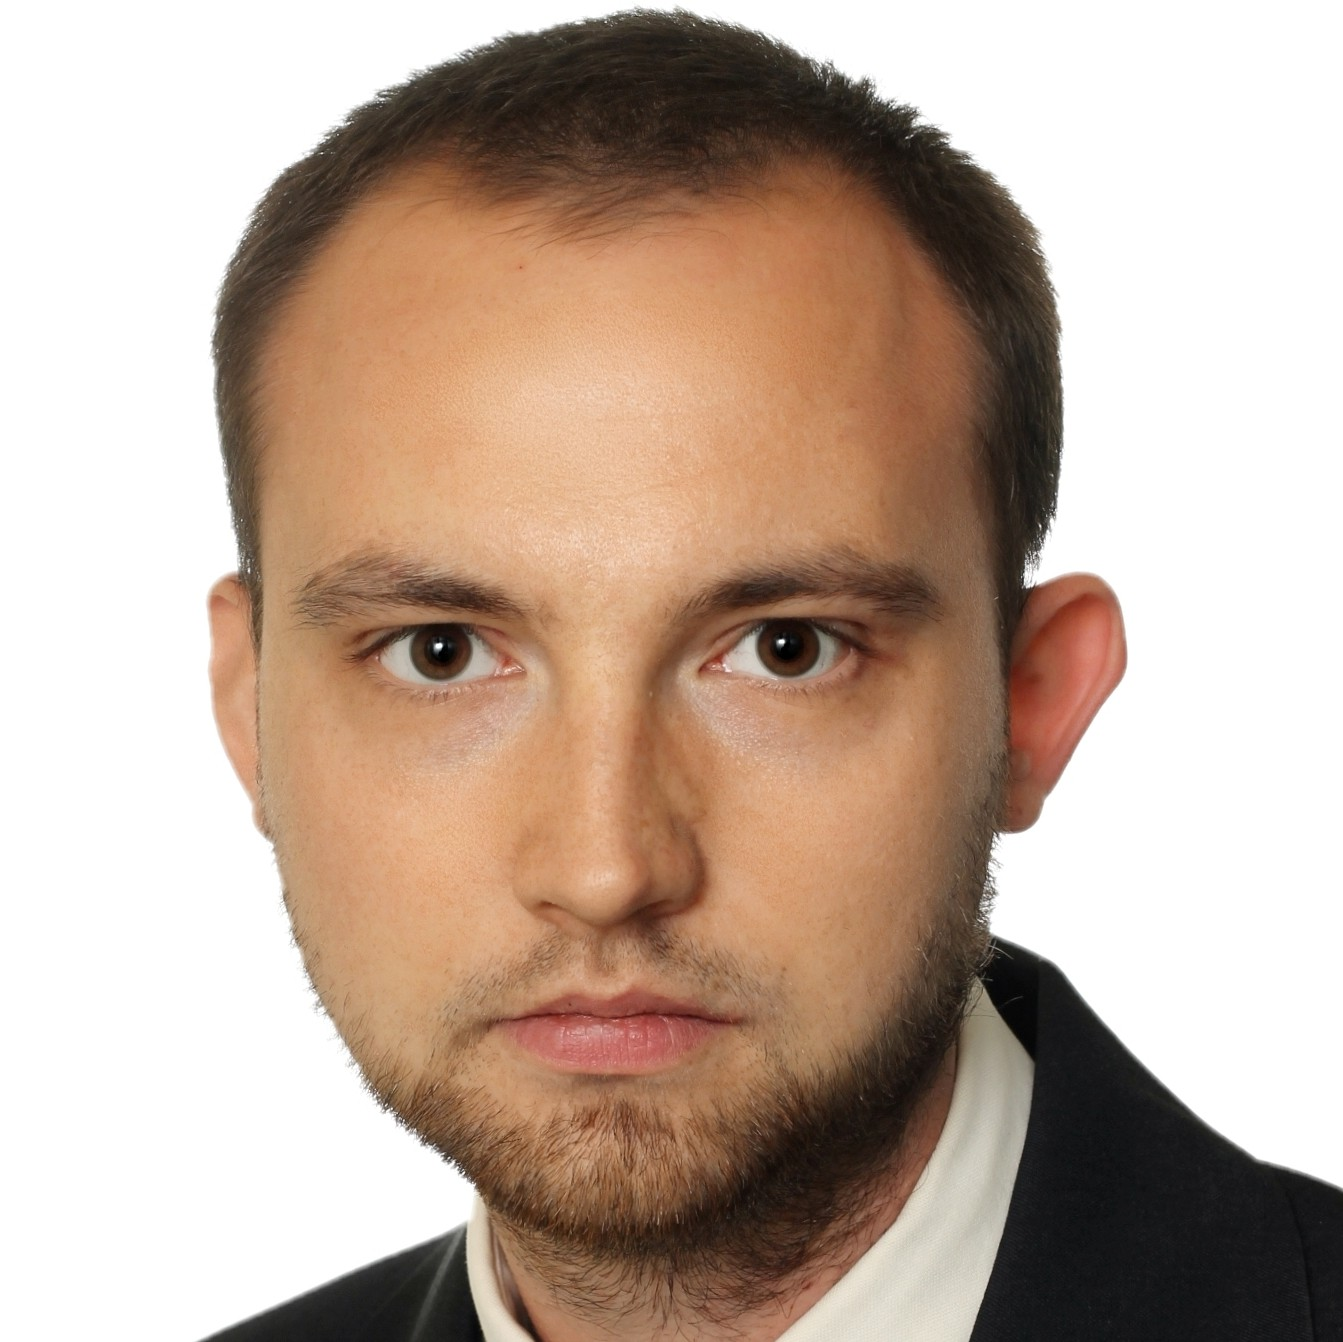
\includegraphics[height=0.2\textheight]{figure/lukasz_chojnacki.jpg} \\
  \textbf{Łukasz}\\\textbf{Chojnacki}\\
  Science
  
\end{minipage}

\column{0.25\textwidth}
\begin{minipage}[c][0.45\textheight][c]{\linewidth}
\centering
    \begin{table}[H]
    \centering
    \begin{tabular}{c}
    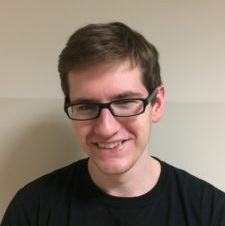
\includegraphics[height=0.2\textheight]{figure/aleksander_bojda.jpg}\\
    \textbf{Aleksander}\\\textbf{Bojda}\\
    Software
    \end{tabular}
    \end{table}
\end{minipage}

\begin{minipage}[c][0.3\textheight][c]{\linewidth}
  \centering
    
\includegraphics[height=0.2\textheight]{figure/jakub_kielar.JPG} \\
    \textbf{Jakub}\\\textbf{Kielar}\\
    Thermal analysis
\end{minipage}

\column{0.25\textwidth}
\begin{minipage}[c][0.45\textheight][c]{\linewidth}
\centering
    \begin{table}[H]
    \centering
    \begin{tabular}{c}
    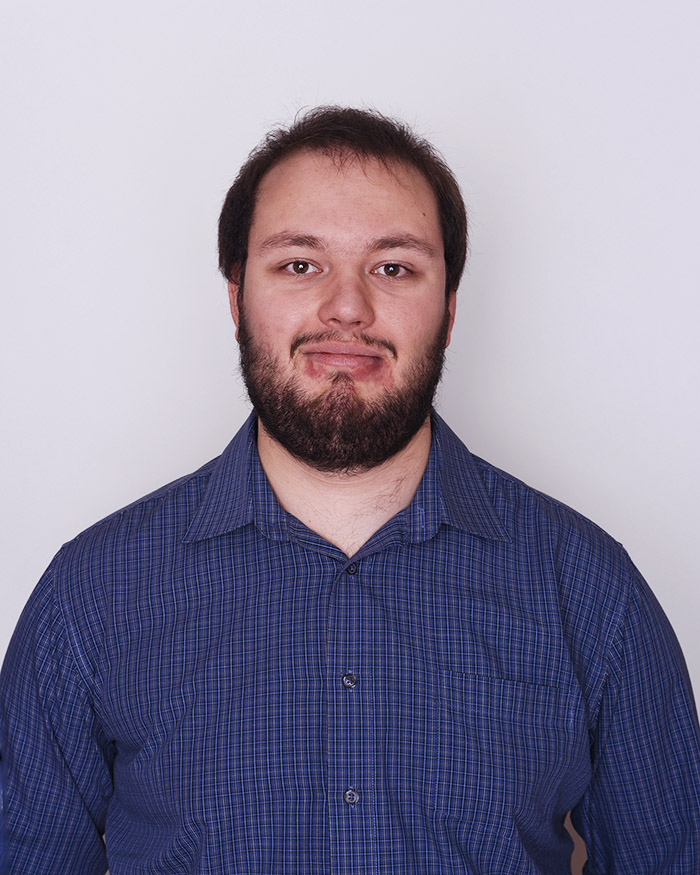
\includegraphics[height=0.2\textheight]{figure/tuzik.jpg}\\
    \thead{Aleksander\\Tuzik}\\Research
    \end{tabular}
    \end{table}
\end{minipage}
\begin{minipage}[c][0.3\textheight][c]{\linewidth}
  \centering
    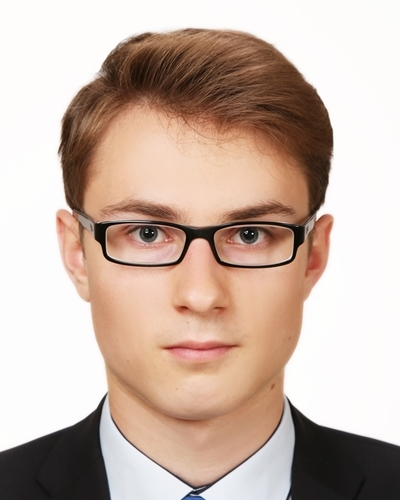
\includegraphics[height=0.2\textheight]{figure/Maciek.jpg} \\
    \textbf{Maciej}\\\textbf{Draguła}\\
    Software
\end{minipage}

\end{columns}	
\end{frame}%koniec slajdu

\begin{frame}
\frametitle{Team structure}
	\centering
    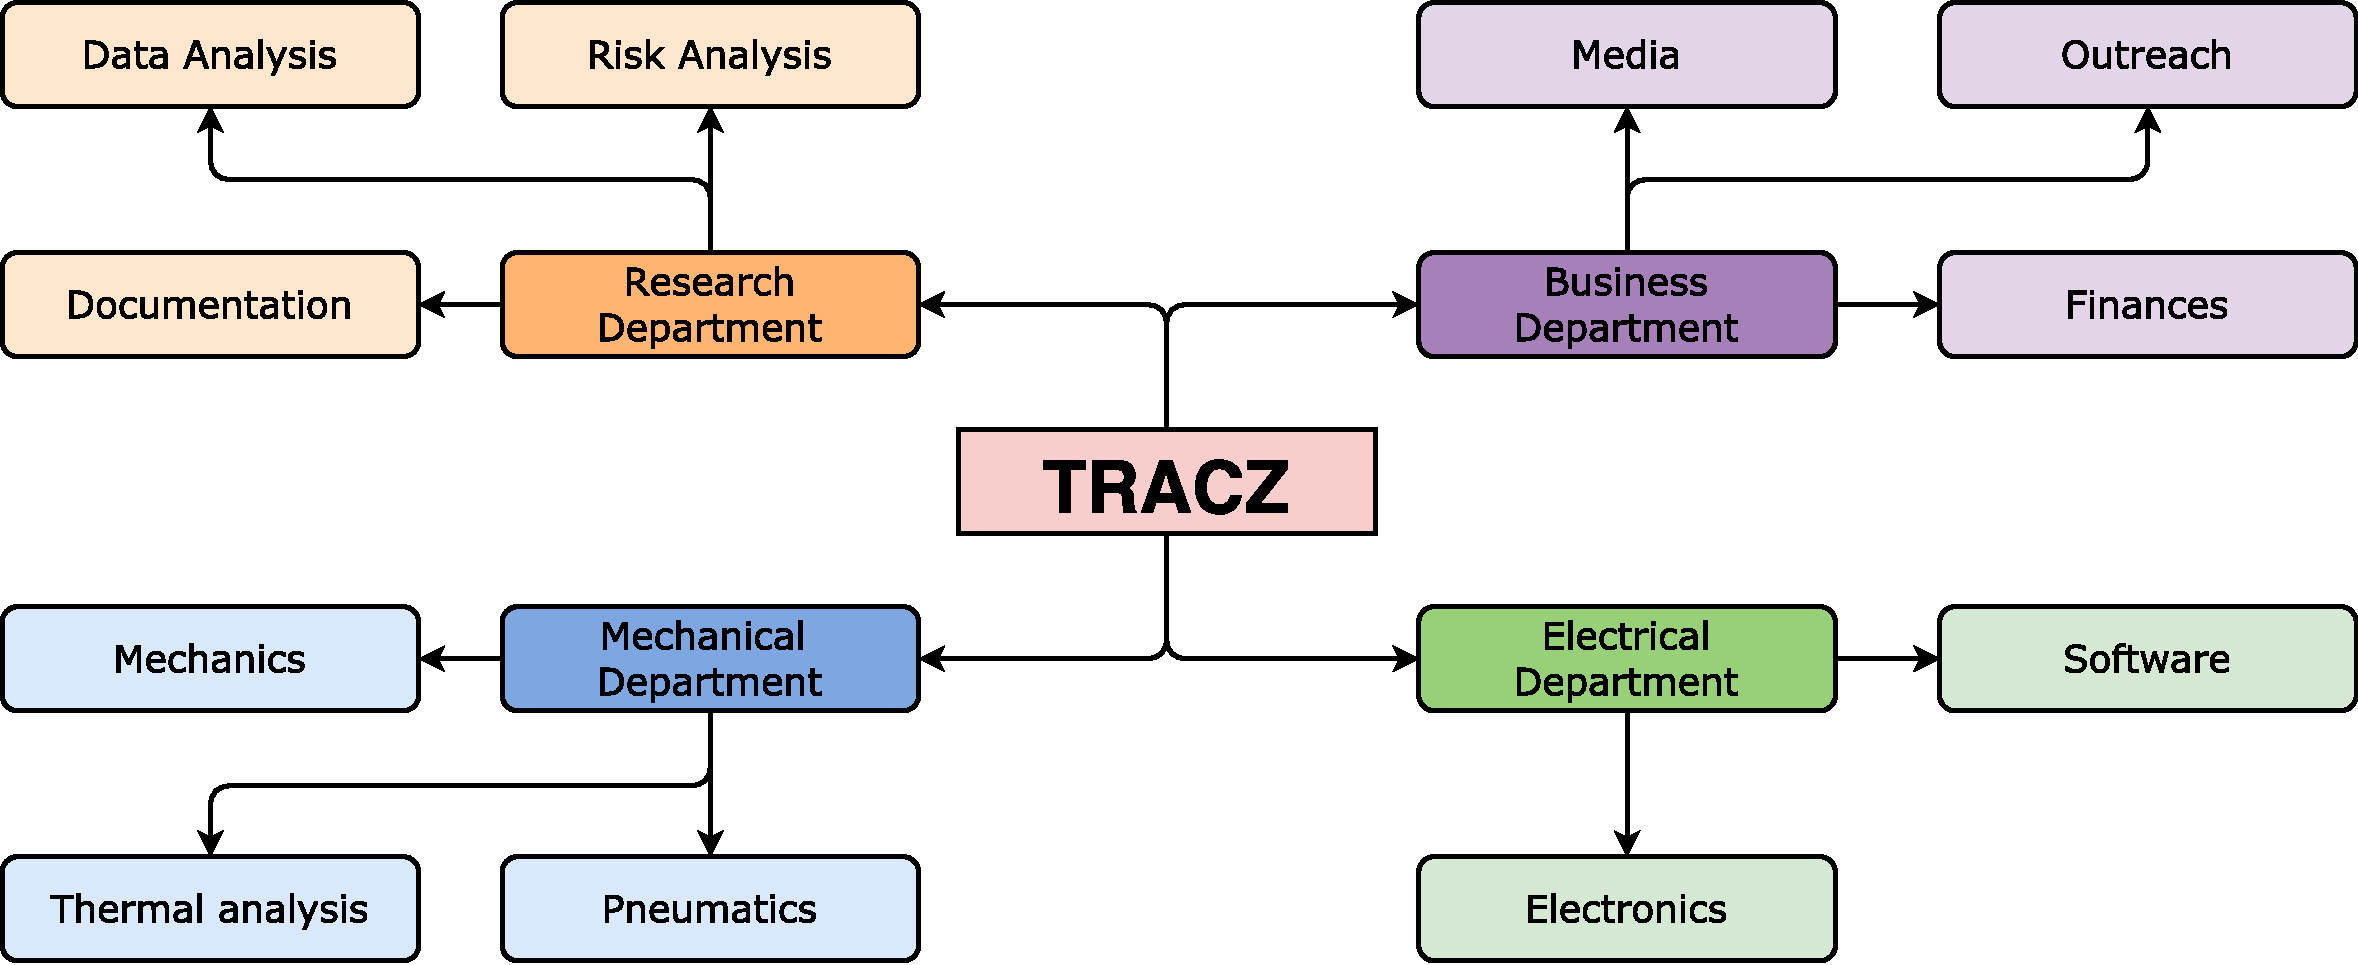
\includegraphics[width=\textwidth]{figure/TraczTeam.pdf}
\end{frame}

%%%%%%%%%%%%%%%%%%%%%%%%%%%%%%%%%%%%%%%%%%%%%%%%%%%%%%%%%%%%%%%%%%%%%%%%%%%%%%%%%%%%%%%%%%%%%%%%%%%%%%

\section{Design}

\begin{frame}
\frametitle{Agenda}
\tableofcontents[currentsection]
\end{frame}

\subsection{Experiment design}
\begin{frame}
\frametitle{Experiment scheme}
  \centering
  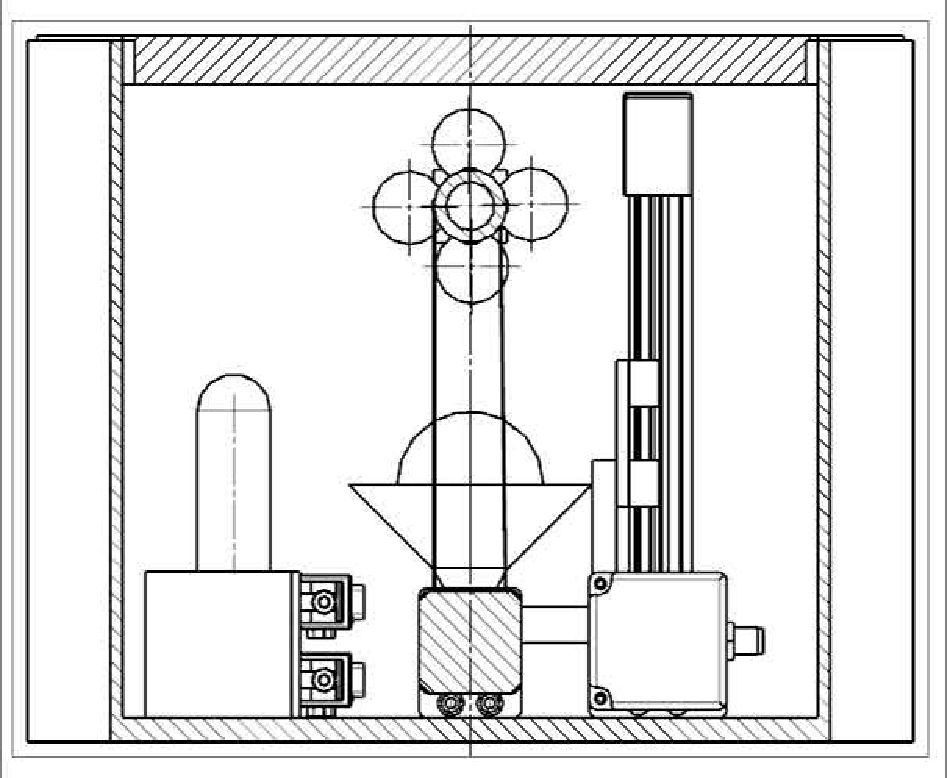
\includegraphics[height=0.9\textheight]{figure/rys_schemat.pdf}	
\end{frame}

%Najpierw mechanical design
%Pozniej pneumatyka
%Elektronika
%Software


\subsection{Mechanics}
\begin{frame}
\frametitle{Mechanical design}
  \centering
  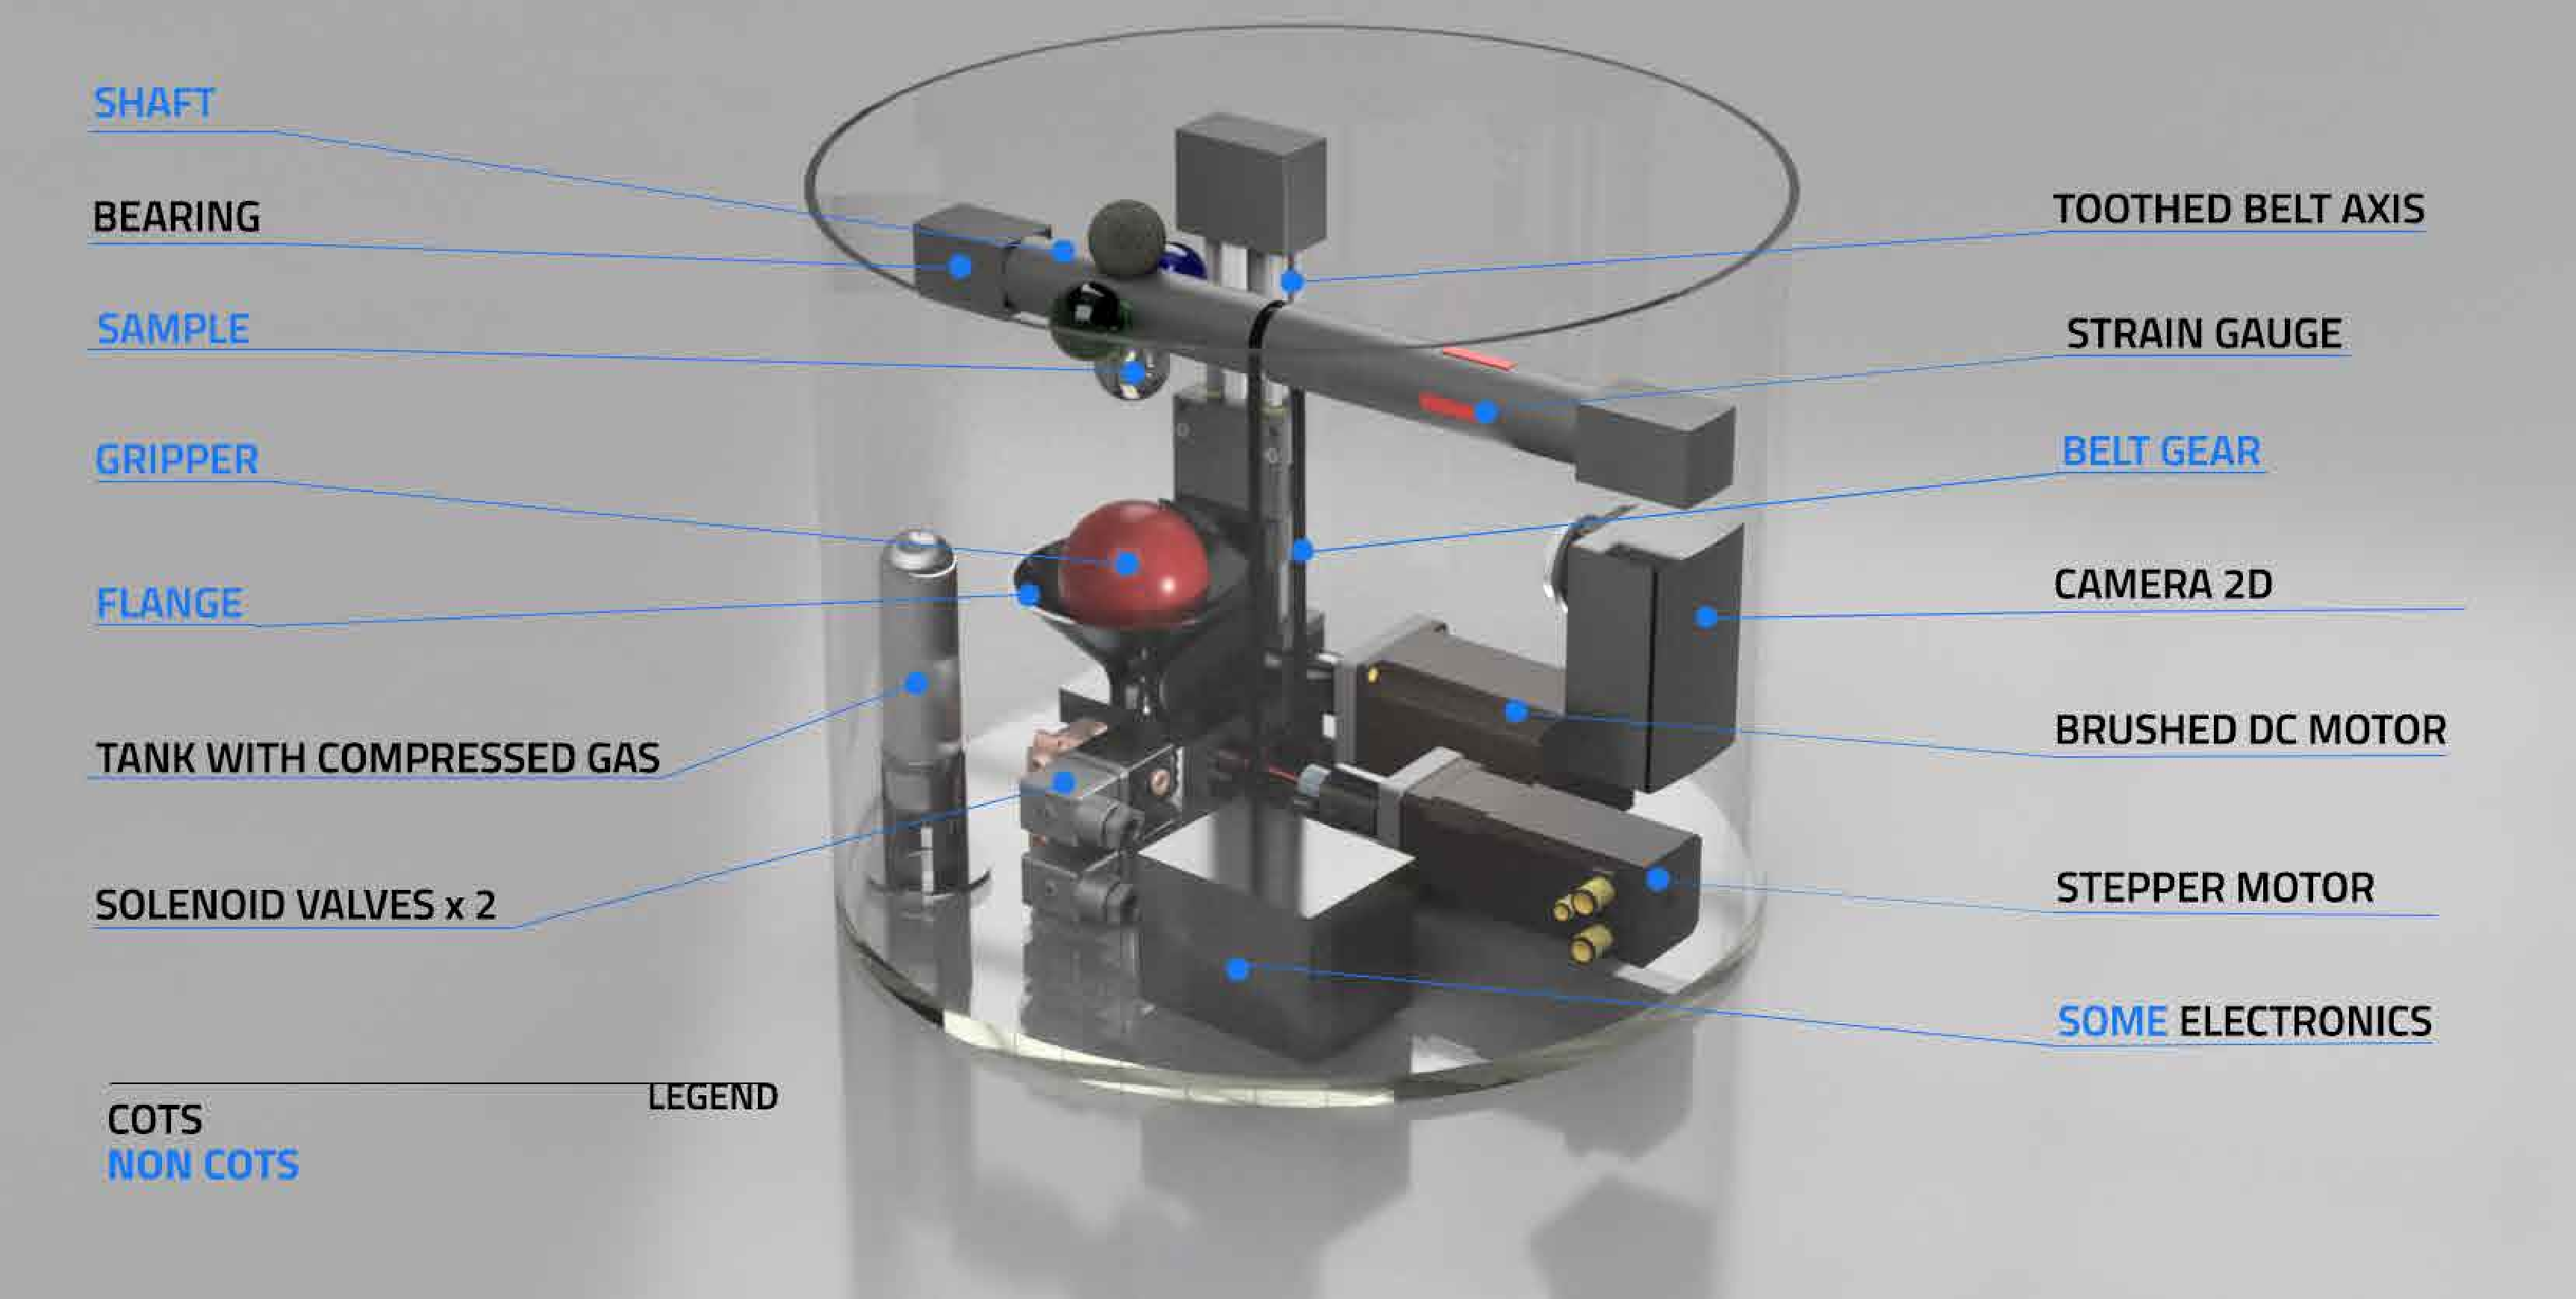
\includegraphics[width=\linewidth]{figure/Modul_v3.pdf}
\end{frame}


\subsection{Pneumatic system} % 
\begin{frame} %początek slajdu
\frametitle{Scheme of the pneumatic system}
\centering {
	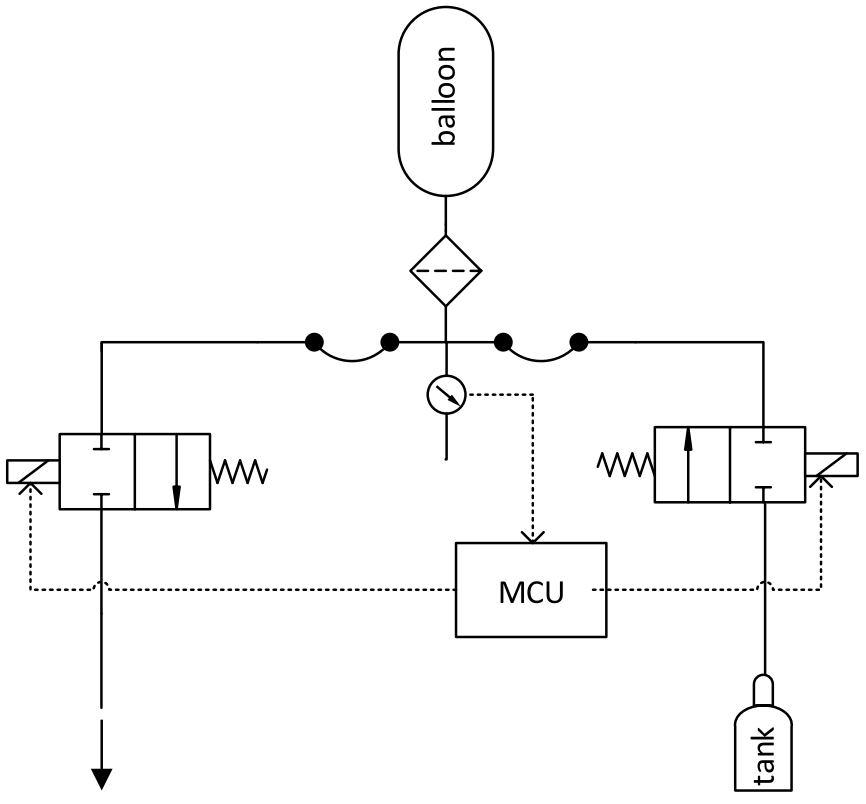
\includegraphics[width=0.7\linewidth]{figure/pneumatic.png}\\
%	\textbf{Scheme of the pneumatic system}\\
	}
\end{frame}%koniec slajdu


\subsection{Electronics} % 
\begin{frame} %początek slajdu
\frametitle{Electronics -- Block diagram}

\centering {
	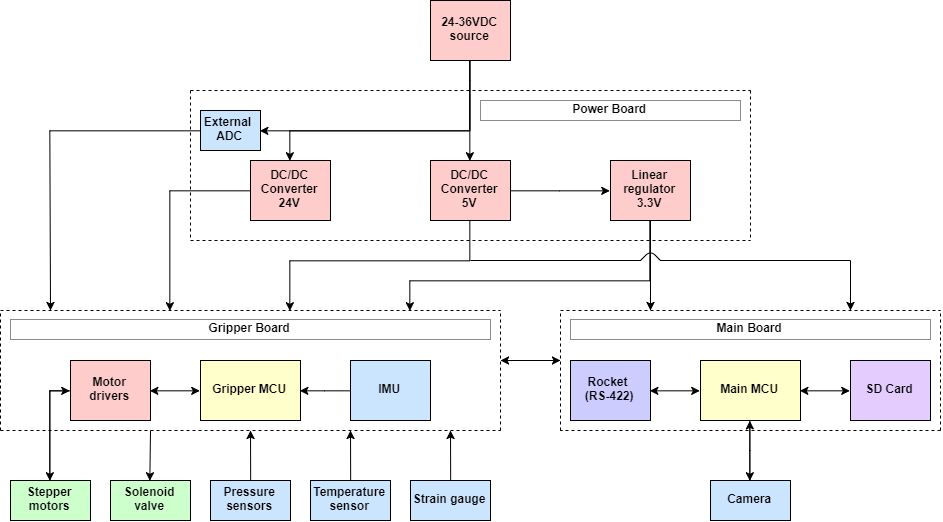
\includegraphics[width=\textwidth]{figure/REXUS_Electronic_design.png}\\
	%\textbf{Block diagram of electronics}\\
	}

\centering
\end{frame}%koniec slajdu

\subsection{Design summary}
\begin{frame}
\frametitle{Design summary}
  \centering
  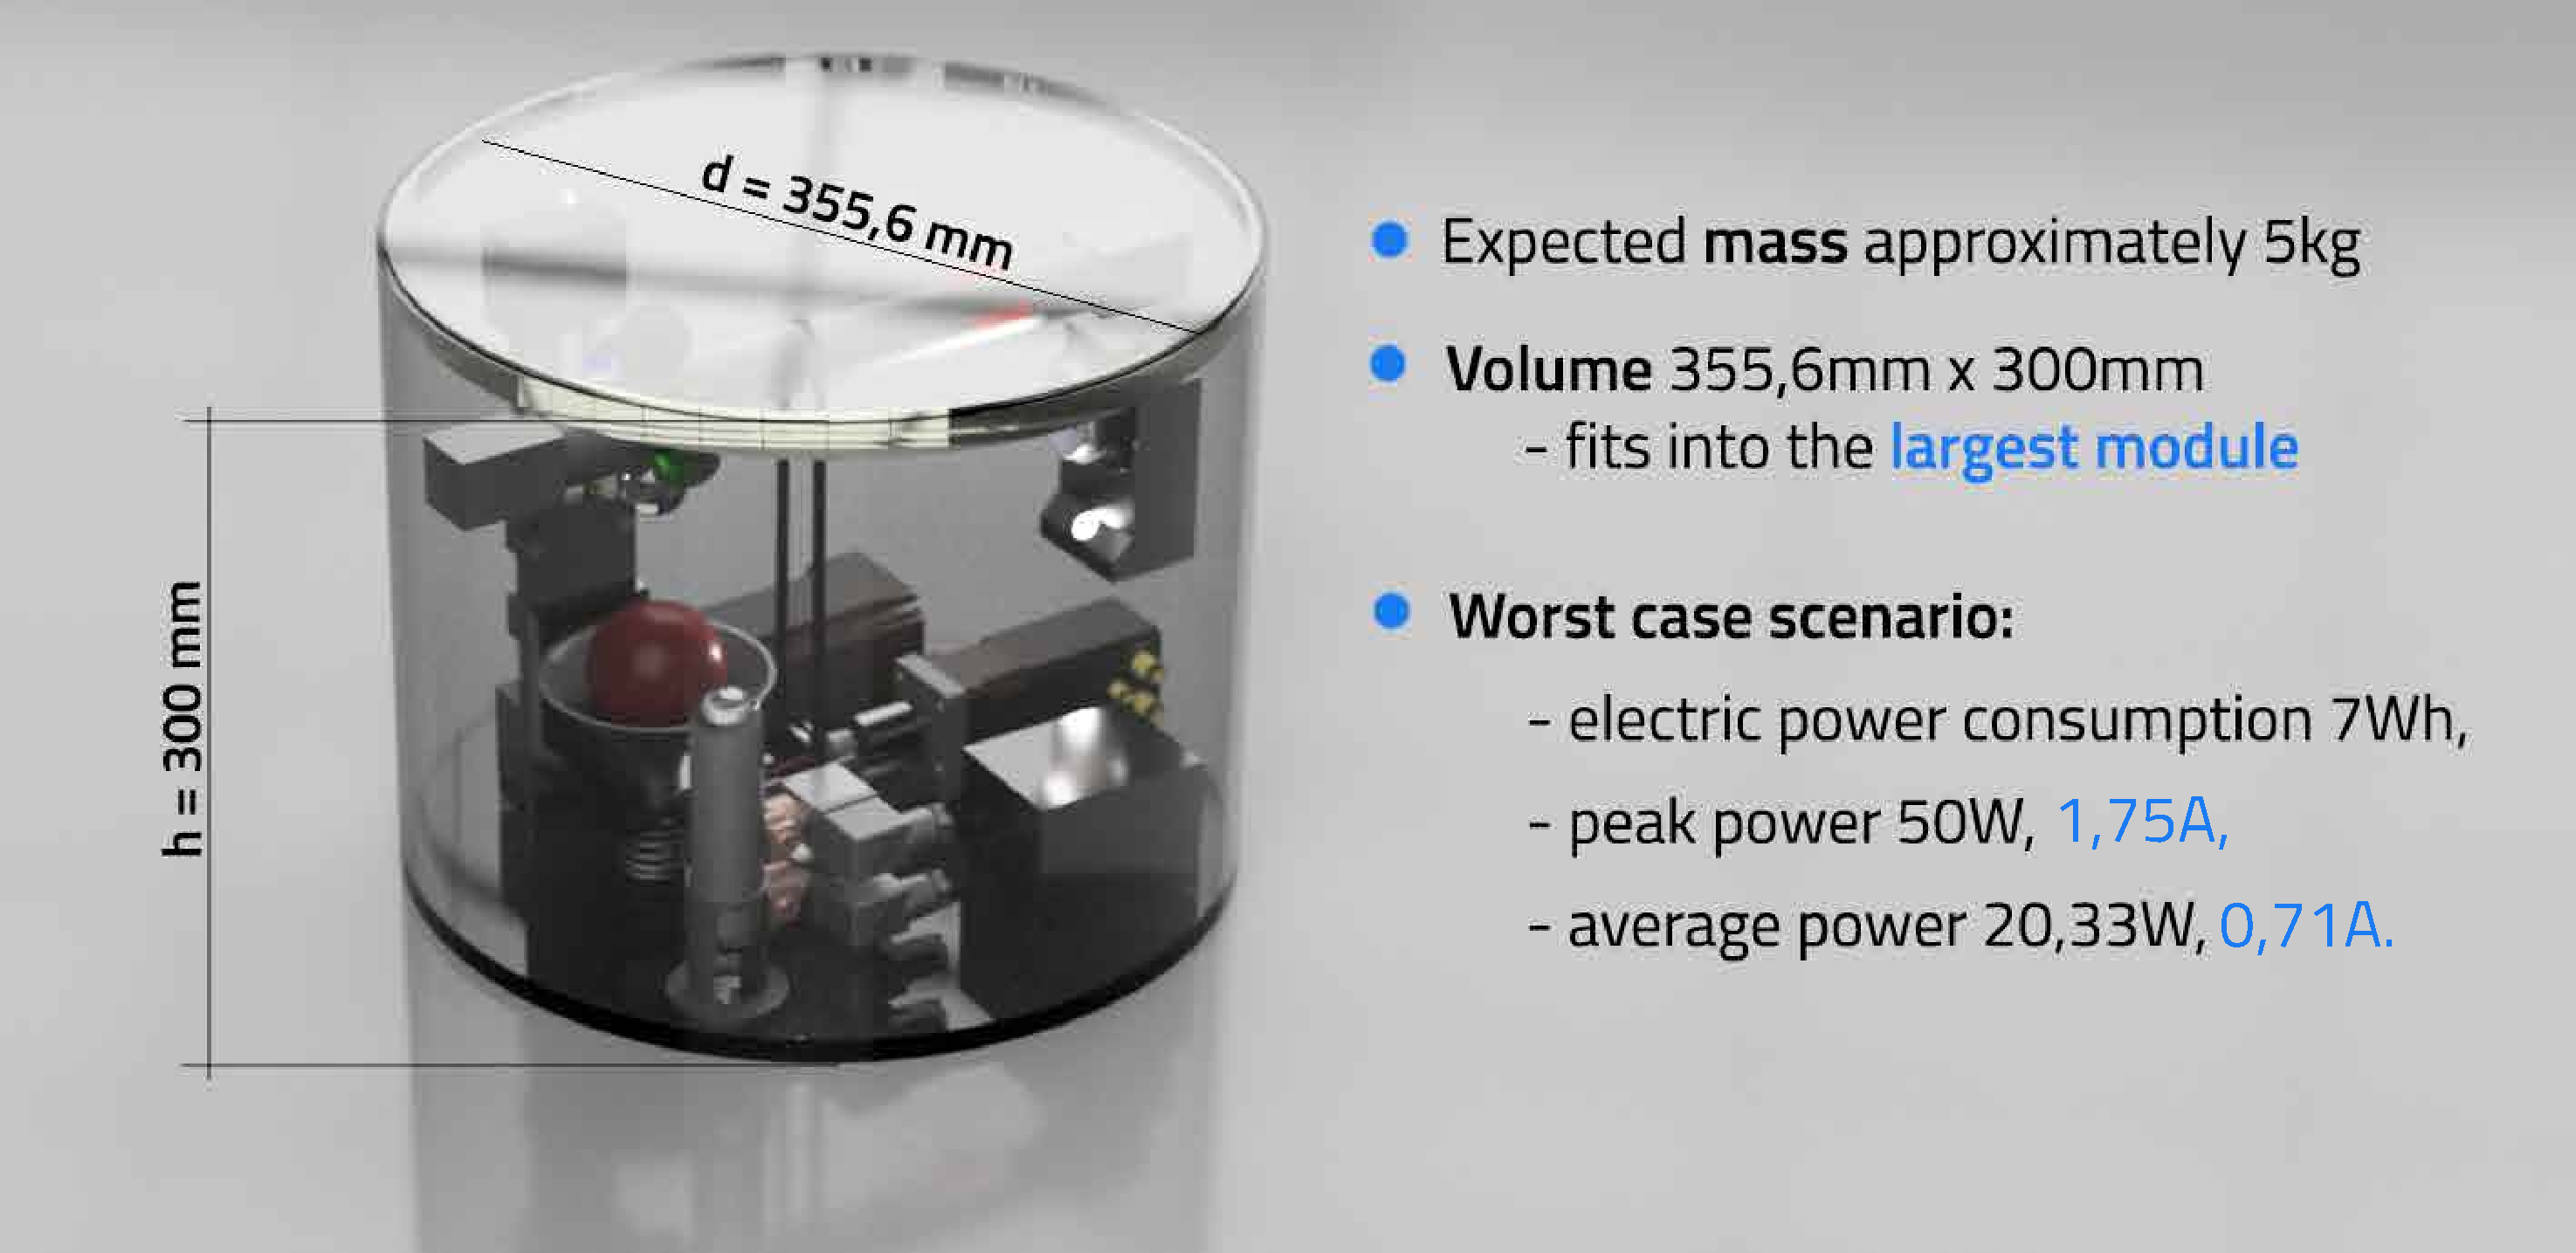
\includegraphics[width=\linewidth]{figure/Modul_SUMMARY.pdf}
\end{frame}

\subsection{Experiment flow}
\begin{frame}
\frametitle{Experiment flow}
% \centering 
\begin{multicols}{2}
{
\hspace{1cm}
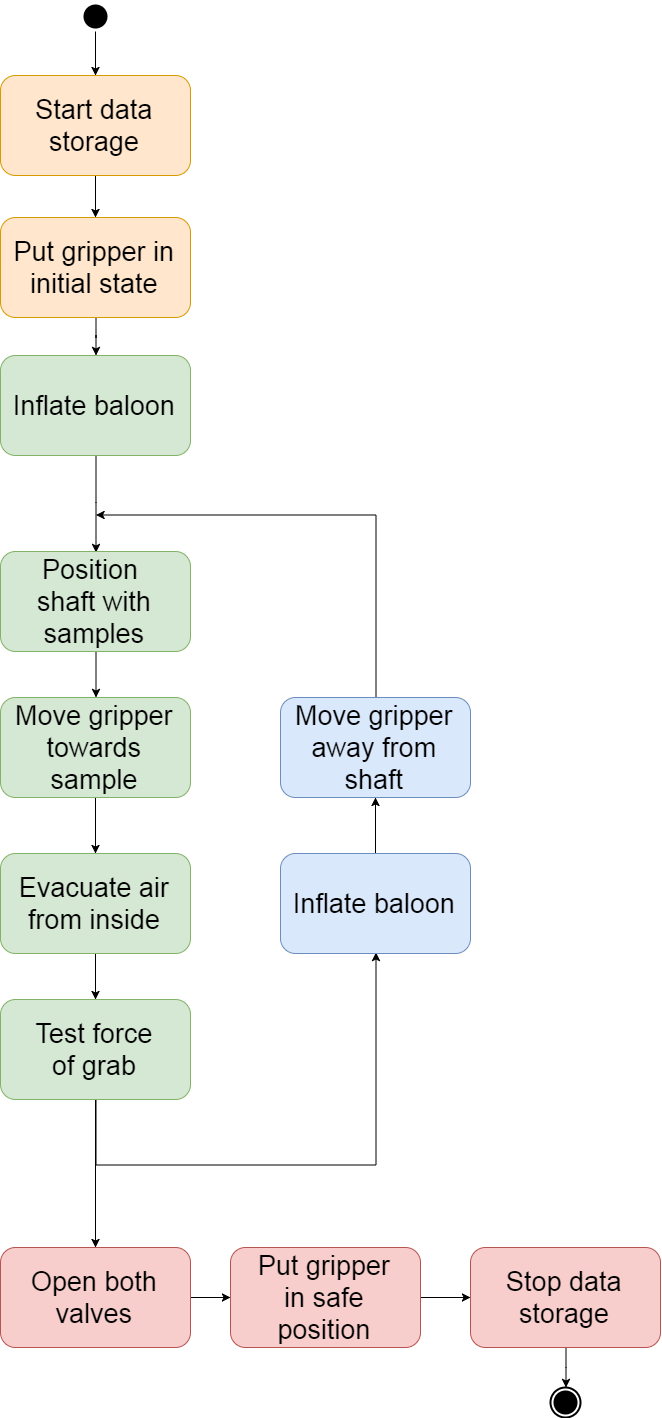
\includegraphics[height=0.8\textheight]{figure/FlowDiagram.png}
}

{
\pause
\textbf{\small Initial state}
\begin{itemize}
\item \small Gripper positioned in a collar
\item \small Gripper-to-vacuum valve open
\item \small Shaft positioned on first sample
\end{itemize}
\pause
\vspace{0.3cm}

\textbf{\small End of the grip}
\begin{itemize}
\item \small Force limit
\item \small Lose of a grip
\item \small Time
\end{itemize}
\pause
\vspace{0.3cm}

\textbf{\small Data flow}
\begin{itemize}
\item \small Gripper board $\Rightarrow$ Main MCU
\item \small SD card
\item \small Downlink
\end{itemize}
}

\end{multicols}

\end{frame}


% \begin{frame}
% \frametitle{Commercial Off The Shelf (COTS) components} %można to ująć bardziej ogólnie
% 	\begin{itemize}
%       \item Positioning shaft motor (encoder) DryLin ® NEMA 17 
%       \item Guide and gripper motor DryLin ® NEMA 23
%       \item Linear Slide Table DryLin ® ZLW 0630 
%       \item 2D camera mvBlueLYNX-X 
%      % \item CO2 38g threaded cartridge (pressurized tank) (nie idziemy w to CO2)
%       \item Gas cylinder-to-Gripper and Gripper-to-Vacuum Solenoid Valves
% %       \item Gas cylinder-TO-Gripper Solenoid Valve HP-DA 1/4'' High Pressure brass FKM 0-75bar 24V DC HP-DA014B010F-024DC 
% %       \item Gripper-TO-Vacuum Solenoid Valve DF-SA 1'' Stainless Steel FKM 0-6bar 24V DC DF-SA100S250F-024DC 
%       \item Lighting for camera High Power Led 1 W WLW28-140-XX1-Px 
%       \item microcontrollers STM32F4 (communication, MCU) and STM32F3 (sensors)
%       \item temperature sensor SMD TMP116NAIDRVR
%       \item Stepper motor driver HY-DIV268N-5A and AMIS-30543 
%       \item Strain gauges, pressure sensors, IMU – 6-axis
% 	\end{itemize}	
% \end{frame}

% \begin{frame} 
%     \frametitle{nonCOTS components}
% 	\begin{itemize}
%     \item different parts of the gripper:
%     \begin{itemize}
%       \item a membrane/balloon 
%       \item a granular material 
%       \item a flange/collar
%     \end{itemize}
% 	\item objects to grip 
% 	\end{itemize}
		
% \end{frame}
%%%%%%%%%%%%%%%%%%%%%%%%%%%%%%%%%%%%%%%%%%%%%%%%%%%%%%%%%%%%%%%%%%%%%%%%%%%%%%%%%%%%%%%%%%%%%%%%%%%%%%

\section{Organisation}

\begin{frame}
\frametitle{Agenda}
\tableofcontents[currentsection]
\end{frame}

\subsection{Data analysis}
\begin{frame}
\frametitle{Data analysis}
    \begin{itemize}
    	\item Calculate and compare grip force from the strain and momentum measurements\vspace{3mm}
        \item Compare results of the experiment with the data collected from the on-ground test\vspace{3mm}
        \item Observe and analyze the behavior of the granulate inside the gripper in microgravity and vacuum
     \end{itemize}
\end{frame}



%%%%%%%%%%%%%%%%%%%%%%%%%%%%%%%%%%%%%%%%%%%%%%%%%%%%%%%%%%%%%%%%%%%%%%%%%%%%%%%%%%%%%%%%%%%%%%%%%%%%%%


\subsection{Costs and fundings}
\begin{frame} %początek slajdu
\frametitle{Costs and fundings}
  \begin{itemize}
    \item Estimated experiment cost with emergency COTS elements \textbf{(+50\%)} \\
    \centering
    \textbf{2400 EUR (+1200 EUR) = 3600 EUR} 
    	\pause
        \vspace{1cm}
    \item Fundings from NzN 2.0 grant - \textbf{5000 EUR} for hardware and\\ \textbf{25000 EUR} for travels, trainings, workshops, conferences 
  \end{itemize}
  
 	\centering	
    
\includegraphics{figure/mnisw.png}
\end{frame}



\subsection{Support and outreach}
\begin{frame}
\frametitle{Support}

\includegraphics[width=\textwidth]{figure/tracz_sponsorzy.png}
\end{frame}

\begin{frame}
\frametitle{Outreach}
\centering

\includegraphics[width=0.8\textwidth]{figure/outreach.png}
\end{frame}

\section*{Ending}
\subsection*{Questions}

\begin{frame}
\frametitle{Questions}
  \centering
\Huge Thank you for attention

\includegraphics[height=0.7\textheight]{figure/logoTRACZ.pdf}
% 	Slajd końcowy - pytania?


\end{frame}



%koniec slajdu

%%%%%%%%%%%%%%%%%%%%%%%%%%%%%%%%%%%%%%%%%%%%%%%%%%%%%%%%%%%%%%%%%%%%%%%%%%%%%%%%%%%%%%%%%%%%%%%%%%%%%%

\appendix


\begin{frame}
\frametitle{WCS Power Consumption Estimation}
\centering
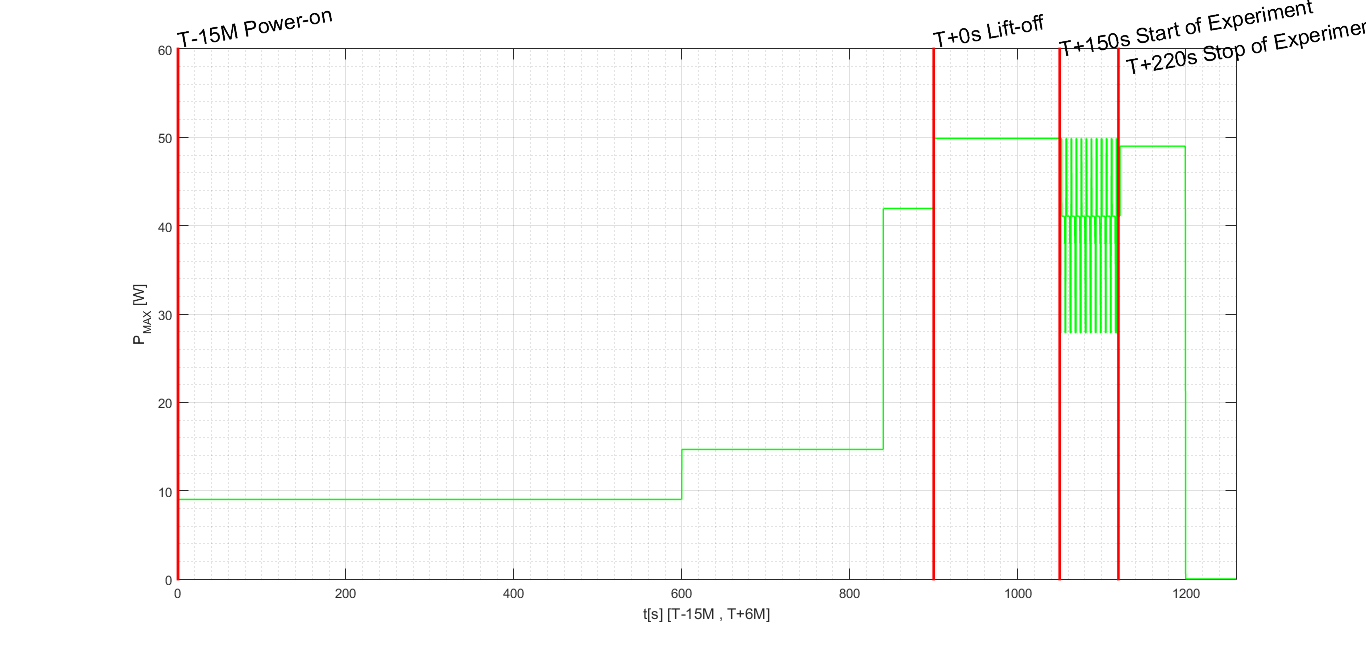
\includegraphics[width=\linewidth] {figure/PeakConsumptionDiagram.png}
\end{frame}

\begin{frame}
\frametitle{Calculation of the required tank volume}
\centering
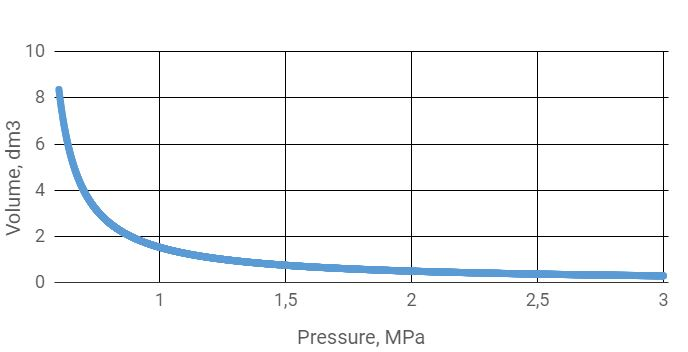
\includegraphics[width=\linewidth] {figure/TANK.JPG}
\end{frame}

\begin{frame}
\frametitle{Different gripping modes}
\centering
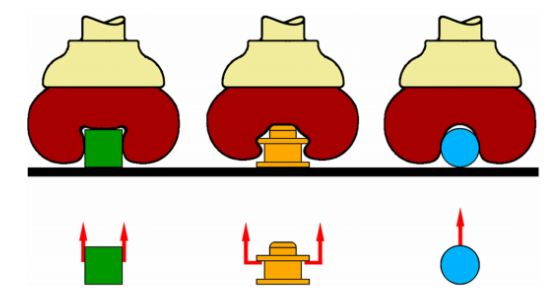
\includegraphics[width=\linewidth] {figure/catching.JPG}
\end{frame}


\begin{frame}[allowframebreaks]
        \frametitle{Appendix -- References}
        \nocite{*} 
        \bibliographystyle{amsalpha}
        \bibliography{biblio}
\end{frame}
	

\end{document}